\documentclass{beamer}

\DeclareMathOperator*{\argmax}{arg\,max}

\usepackage{graphicx}

\usepackage[noend]{algpseudocode}
\renewcommand{\algorithmicrequire}{\textbf{Input:}}
\renewcommand{\algorithmicensure}{\textbf{Output:}}

\usepackage{listings}
\lstset{basicstyle=\tiny}

\usetheme{Madrid}

\hypersetup{pdfpagemode=FullScreen}

\begin{document}

\title[Parallel Simulation R\&S Procedures]
{
Design and Implementation of Parallel Simulation~Ranking~and~Selection~Procedures
}
\author{WU, Yang}
\institute[IELM, HKUST]
{
  Department of Industrial Engineering and Logistics Management\\
  The Hong Kong University of Science and Technology
}
\date{2, Aug 2013}

\begin{frame}
\titlepage
\end{frame}

\begin{frame}
\frametitle{Outline}
\tableofcontents
\end{frame}

\AtBeginSection[]
{
  \begin{frame}
  \frametitle{Outline}
  \tableofcontents[currentsection]
  \end{frame}
}

\section{Introduction}

\begin{frame}
\frametitle{Original Problem}
\framesubtitle{Problem of Selecting the Best}
\begin{itemize}
\item decide the best one from a finite number of alternatives
\vspace{\baselineskip}
\item the best is defined as the one with the largest or smallest mean, inferred from statistical sampling
\vspace{\baselineskip}
\item sampling by real experiments or computer simulations
\end{itemize}
\end{frame}

\begin{frame}
\frametitle{Original Solution}
\framesubtitle{within Serial Computing Environment}
\begin{itemize}
\item Simulation Ranking-and-Selection(R\&S) Procedures
\begin{itemize}
\item a black-box approach
\item simulate against all the alternatives, each for many times
\item collect enough samples and make our decision
\item statistical guarantees of correct selection
\end{itemize}
\vspace{\baselineskip}
\item Serial Simulation R\&S Procedures
\begin{itemize}
\item run simulation, get corresponding sample, do some calculation
\item starts earlier, finish earlier: "the sequential nature"
\item statistical validity of serial procedure
\end{itemize}
\end{itemize}
\end{frame}

\begin{frame}
\frametitle {Significant Change of Computing Environment}
\framesubtitle{The Age of Parallel Computing}
\begin{itemize}
\item fast-growing of serial computing speed has almost stopped, due to physical limitations
\vspace{\baselineskip}
\item growing of computing power relies on available parallel execution units
\vspace{\baselineskip}
\item large problem can be divided into smaller ones, and small problems can be executed simultaneously, thus speeding up
\end{itemize}
\end{frame}

\begin{frame}
\frametitle {Significant Change of Computing Environment}
\framesubtitle{from Serial to Parallel}
\begin{itemize}
\item Before the Age of Parallel Computing
\begin{itemize}
\item program will execute faster as the serial computing speed goes up
\item simulation R\&S procedures will speed-up with the developing of computing technology naturally, without modifying the design of procedure, even the implementation
\end{itemize}
\vspace{\baselineskip}
\item During the Age of Parallel Computing
\begin{itemize}
\item serial program will {\color{blue} NOT} execute faster with more available parallel execution units, unless get paralleled, explicitly or implicitly
\item serial simulation R\&S procedures will {\color{blue} NOT} speed-up with the developing of computing technology, unless re-designed and implemented into parallel
\end{itemize}
\end{itemize}
\end{frame}

\begin{frame}
\frametitle{Extra Consideration of Computing}
\framesubtitle{from Complexity to Scalability}
\begin{itemize}
\item {\bf performance}
\begin{itemize}
\item {\bf response time:} time cost per job
\item {\bf throughput:} number of jobs done per time unit
\end{itemize}
\item {\bf time complexity}
\begin{itemize}
\item evaluate the serial algorithm performance against the increasing of problem size
\item independent of serial execution speed
\end{itemize}
\item {\bf scalability}
\begin{itemize}
\item evaluate the system performance against the increasing of computing resource
\item also independent of serial execution speed
\item extremely important, in the sense that we can get better performance almost immediately simply by adding more computing resources
\end{itemize}
\end{itemize}
\end{frame}

\begin{frame}
\frametitle{Our Work}
\begin{itemize}
\item We design and implement a parallel framework for simulation R\&S procedures, with master-slave structure in higher level, and achieves a good scalability illustrated in numerical experiments.
\vspace{\baselineskip}
\item Based on this framework, we design and implement several specific simulation experiments and R\&S procedures, which has demonstrated the good extensibility of our framework.
\vspace{\baselineskip}
\item Within specific R\&S procedure, we decrease the serial algorithm time complexity, by adopting heap, a widely used data structure. This also help improve the performance of the whole system.
\end{itemize}
\end{frame}

\section{Parallelism Analysis}

\begin{frame}
\frametitle{Parallelism Analysis}
\framesubtitle{A Staged Procedure: the Rinott's Procedure}
\begin{enumerate}
\item{Set up: } Set up parameters $\alpha$, $\delta$ and $n_0$. $n_0$ is the sample size in first stage and $n_0 \geqslant 2$.
\item{Initialize: } Calculate Rinott's constant $h$ with $n_0, k, \alpha$. Collect $n_0$ independent sample values $X_{ij}$, where $j = 1, 2,...,n_0$, for each alternative $i$, by repeatedly running simulation experiments against that alternative, and for $i = 1, 2,...,k$, calculate $S_i^2$. Let 
$ N_i = \max\{n_0, \lceil \frac{h^2S_i^2}{\delta^2} \rceil\} $ where $N_i$ is the number of sample value that will eventually taken from alternative $i$.
\item{Stopping Rule: } If $n_0 \geqslant \max N_i$ then stop and select the alternative with the best sample mean, namely the largest or smallest $\bar{X_i(n_0)}$. Else take $\max\{N_i - n_0, 0\}$ extra sample values from each alternative $i$ by continue repeating the simulation experiments, after which select the alternative with largest or smallest $\bar{X_i(N_i)}$ as the best.
\end{enumerate}
\end{frame}

\begin{frame}
\frametitle{Parallelism Analysis}
\framesubtitle{A Fully Sequential Procedure: the KN Procedure}
\begin{enumerate}
\item{Set up: } Set up parameters $\alpha$, $\delta$, $n_0$ and $h^2 = (n_0 -1)[(\frac{2\alpha}{k - 1})^{-2/(n_0-1)} - 1]$.
\item{Initialize: } Collect $n_0$ independent sample values $X_{i\ell}$, where $\ell = 1, 2,...,n_0$, for each alternative $i$, by repeatedly running simulation experiments against that alternative, and for $i \neq j$ compute $S_{ij}^2 = \frac{1}{n_0 - 1}\sum_{\ell=1}^{n_0}(X_{i\ell} - X_{j\ell} - [\bar{X_i}(n_0) - \bar{X_j}(n_0)]^2)$, let $r = n_0$.
\item{Elimination: } Set $I^{old} = I$. Let $I = I^{old} - \{i \in I^{old}: \bar{X}_{i\ell}(r) - \bar{X}_{j\ell}(r) < \min\{0, - \frac{h^2S_{ij}^2}{2r\delta} + \frac{\delta}{2} \} \}$
\item{Stopping Rule: } If $|I| = 1$, then stop and select the only surviving alternative, otherwise take another simulation output $X_{i,r+1}$ from each system $i$ and set $r = r + 1$ and go to Elimination.
\end{enumerate}
\end{frame}

\begin{frame}
\frametitle{Redesign of Existing Procedures}
\framesubtitle{Rinott's Procedure}
\begin{algorithmic}[1]
\Require $k, \alpha, \delta, n_0$
\State $h \gets$ the Rinott's const with arguments $k, \alpha, n_0$
\State $altIds \gets \{0, 1, 2...k - 1, 0, 1, 2...k - 1...\}$ \Comment{repeat $n_0$ cycles}
\State simulate alternatives with id in $altIds$ \textbf{in parallel}; store result into $X_{ij}$
\State $altIds2 \gets \emptyset$
\For{$i = 0 \to k - 1$}
  \State $\bar{X_i}(n_0) = \frac{1}{n_0} \sum_{j=0}^{n_0 - 1}X_{ij}$;  $S_i^2 = \frac{1}{n_0 - 1} \sum_{j=0}^{n_0 - 1}(X_{ij} - \bar{X_i}(n_0))^2$;
  \State $N_i = \max\{n_0, \lceil \frac{h^2S_i^2}{\delta^2} \rceil\}$
  \For{$j = 0 \to (N_0 - n_0) - 1$}
    \State append $i$ into $altIds2$
  \EndFor
\EndFor
\State simulate alternatives with id in $altIds2$ \textbf{in parallel}; store result into $X_{ij}$
\For{$i = 0 \to k - 1$}
  \State $\bar{X_i}(N_0) = \frac{1}{N_0} \sum_{j=0}^{N_0 - 1}X_{ij}$
\EndFor
\State \Return $\argmax_{i}\bar{X_i}(N_0)$
\end{algorithmic}
\end{frame}

\begin{frame}
\frametitle{Redesign of Existing Procedures}
\framesubtitle{Vector Filling KN Procedure}
\begin{algorithmic}[1]
\Require $k, \alpha, \delta, n_0$
\State $h^2 \gets (n_0 -1)[(\frac{2\alpha}{k - 1})^{-2/(n_0-1)} - 1]$
\State $altIds \gets \{0, 1, 2...k - 1, 0, 1, 2...k - 1...\}$ \Comment{repeat $n_0$ cycles}
\State simulate against alternatives with id in $altIds$ \textbf{in parallel}; store result into $X_{i\ell}$
\State $survivingCount \gets k$; $r \gets n_0$
\State comparison and elimination
\While{$survivingCount > 1$}
  \State $simOutput \gets $ take one generated simulation output into $X_{i\ell}$
  \State simulate against all surviving alternatives \textbf{in parallel and asynchronously}
  \If{$\min{len(X_i)} > r$}
    \State $r \gets r + 1$; comparison and elimination
  \EndIf
\EndWhile
\State \Return id of the surviving alternative
\end{algorithmic}
\end{frame}

\begin{frame}
\frametitle{Redesign of Existing Procedures}
\framesubtitle{Asymptotic Parallel Sequential Procedure}
\begin{algorithmic}[1]
\Require $k, \alpha, \delta, n_0$
\State $a \gets - \log{[2\alpha / (k - 1)]}$
\State $altIds \gets \{0, 1, 2...k - 1, 0, 1, 2...k - 1...\}$ \Comment{repeat $n_0$ cycles}
\State simulate against alternatives with id in $altIds$ \textbf{in parallel}; store result into $X_{i\ell}$
\State $survivingCount \gets k$; comparison and elimination
\State simulate against all surviving alternatives \textbf{in parallel and asynchronously}, with a phantom alternative p.
\While{$survivingCount > 1$}
  \State $simOutput \gets $ take one generated simulation output into $X_{i\ell}$
  \If{$simOutput is phantom$}
    \State simulate against all surviving alternatives \textbf{in parallel and asynchronously}, with a phantom alternative p.
    \State comparison and elimination
  \EndIf
\EndWhile
\State \Return id of the surviving alternative
\end{algorithmic}
\end{frame}

\section{System Design}

\begin{frame}
\frametitle{System Overview}
\framesubtitle{A Sequence Diagram}
\begin{figure}[ht]
\centering
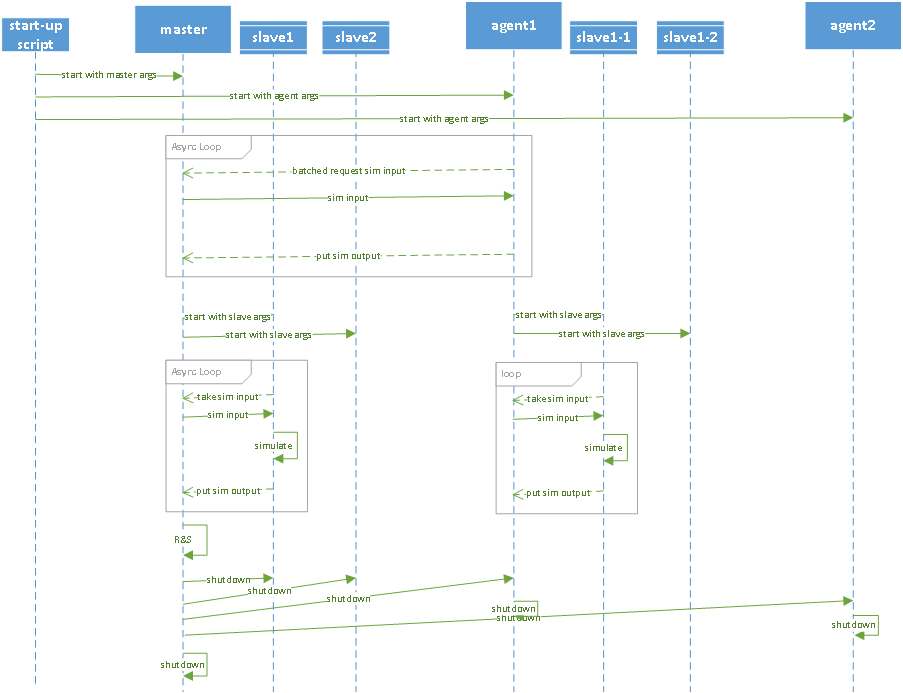
\includegraphics[height=72mm]{overview_seq.png}
\end{figure}
\end{frame}

\begin{frame}
\frametitle{Master-Slave Structure on Single Machine}
\framesubtitle{Communication via FIFO Queue}
\begin{figure}[ht]
\centering
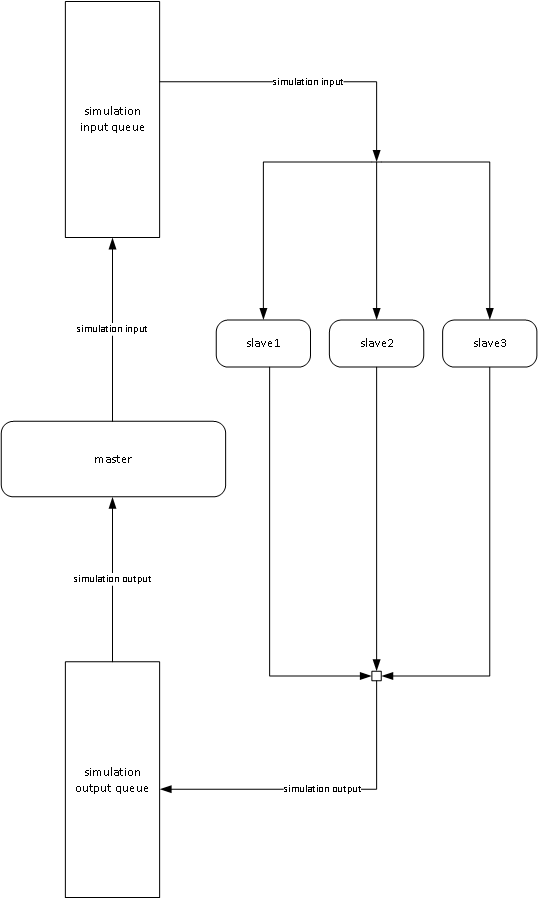
\includegraphics[height=64mm]{master-slave-queue.png}
\end{figure}
\end{frame}

\begin{frame}
\frametitle{Design for Extensibility}
\framesubtitle{Partial Class Diagram}
\begin{figure}[ht]
\centering
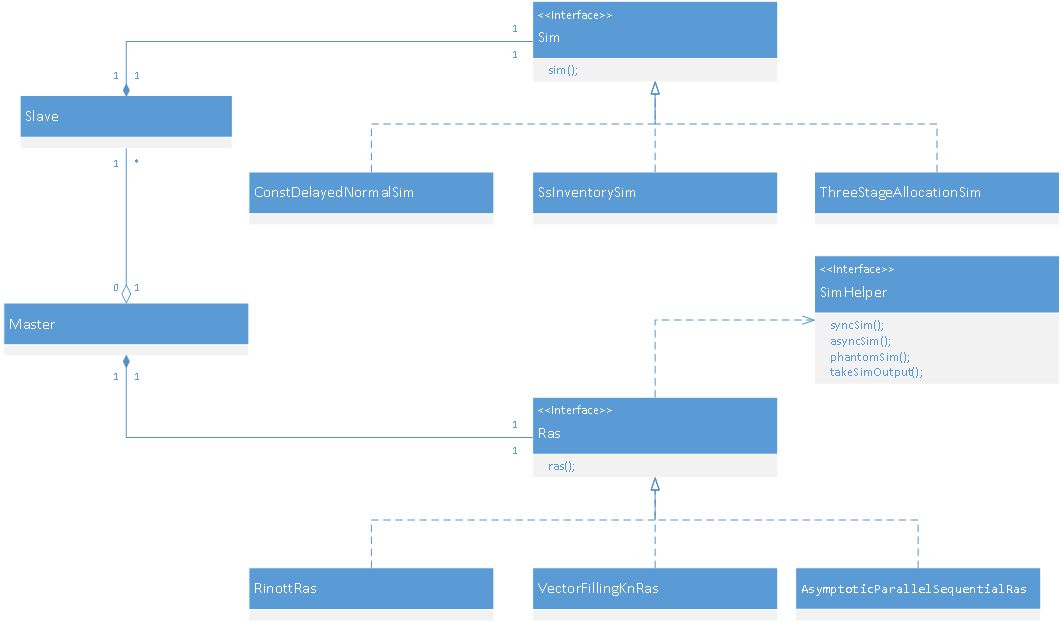
\includegraphics[height=64mm]{ras-sim-class.png}
\end{figure}
\end{frame}

\begin{frame}[fragile]
\frametitle{Design for Extensibility}
\framesubtitle{Interfaces to Implement}
\begin{itemize}
\item Sim interface:
\begin{lstlisting}[language=Java]
public double[] sim(double[] alt, double[] args, long[] seed);
\end{lstlisting}
\vspace{\baselineskip}
\item Ras interface:
\begin{lstlisting}[language=Java]
public int ras(double[][] alts, double[] args, SimHelper helper);
\end{lstlisting}
\end{itemize}
\end{frame}

\begin{frame}[fragile]
\frametitle{Design for Extensibility}
\framesubtitle{SimHelper interface used by implementing Ras interface}
\begin{lstlisting} [language=Java]
public class SimInput
{
  public int altID;
  public double[] args;
  public long[] seed;
}
\end{lstlisting}
\begin{lstlisting}[language=Java]
public class SimOutput
{
  public int altID;
  public double[] result;
}
\end{lstlisting}
\begin{lstlisting}[language=Java]
public interface SimHelper
{
  public SimOutput[] syncSim(int[] altIDs);
  public int asyncSim(int[] altIDs);
  public int phantomSim(int[] altIDs);
  public SimOutput[] takeSimOutputs(int n, boolean block);
}
\end{lstlisting}
\end{frame}

\begin{frame}
\frametitle{Logging Items}
\begin{itemize}
\item selection result
\item response time
\item input sequence
\begin{itemize}
\item $altId, args, seeds$
\item $count for put and take$
\item record of sampling rule
\end{itemize}
\item output sequence
\begin{itemize}
\item $altId, result$, optionally corresponding input info
\item $count for put and take$
\item can be used to "replay" the parallel procedure in serial
\end{itemize}
\end{itemize}
\end{frame}

\begin{frame}
\frametitle{Deploy on Cluster}
\begin{itemize}
\item Scale-up v.s. Scale-out
\item agent in charge of communication via network
\item simulation input management
\begin{algorithmic}[1]
\While{\text{true}}
  \If{$inputQueue.size() < s1$}
    \State{send request for $(s2 - s1)$ simulation inputs via network}
    \ForAll{obtained simulation inputs}
      \State{inputQueue.put(input)}
    \EndFor
  \Else
    \State{sleep for 1 second}
  \EndIf
\EndWhile
\end{algorithmic}
\item simulation output management (as aggressive as possible)
\end{itemize}
\end{frame}

\section{System Evaluation}

\begin{frame}
\frametitle{Comparative Study of Three Parallel Procedures}
\begin{itemize}
\item {Alternative: } normal distributed simulation result, with pre-known mean and variance
\item {Configuration: } 100 alternatives, one of them has max-mean 1, others has mean of 0. Variance is 1.
\item {Environment: } pc with 8 hardware thread, using 4 slaves. $\alpha=0.05, \delta=1, n_0 = 10$, the Rinott's const is 68.2226.
\item {Result: } $100\%$ correct selection.
\end{itemize}
\begin{table}[ht]
\begin{center}
\scalebox{0.6}
{
\begin{tabular}{|c|c|c|c|}
\hline
& Rinott & VFKN & APS \\
\hline
0 & 457533, 457533, 457533, 457533, 3368ms & 23889, 23833, 23832, 3780, 476ms & 1296, 1296, 1296, 1292, 95ms \\
\hline
1 & 467561, 467561, 467561, 467561, 3293ms & 16363, 14981, 14980, 2173, 116ms & 1333, 1333, 1333, 1329, 56ms \\
\hline
2 & 490175, 490175, 490175, 490175, 3356ms & 24061, 17010, 17009, 3050, 138ms & 1265, 1265, 1265, 1262, 47ms \\
\hline
3 & 473949, 473949, 473949, 473949, 3306ms & 16638, 13863, 13862, 2898, 111ms & 1205, 1205, 1205, 1202, 37ms \\
\hline
4 & 446015, 446015, 446015, 446015, 3151ms & 14937, 13771, 13769, 3758, 114ms & 1247, 1247, 1247, 1243, 45ms \\
\hline
\end{tabular}
}
\end{center}
\end{table}
\tiny{In each table cell, the numbers means count of simulation input put, count of simulation input taken, count of simulation output put, count of simulation output taken and total time cost, respectively.}
\end{frame}

\begin{frame}
\frametitle{Scalability on Single Machine}
\begin{itemize}
\item {Alternative: } feasible region of a three-stage allocation problem.
\item {Configuration: } 21660 alternatives, with 2 best one, and 4 acceptable good one, from IZ viewpoint.
\item {Environment: } a powerful server with 48 threads. APS procedure, $\alpha=0.05, \delta=1, n_0 = 10$.
\item {Result: } $100\%$ correct selection.
\begin{table}[ht]
\begin{center}
\scalebox{0.85}
{
\begin{tabular}{|c|c|c|c|c|c|c|}
\hline
Num. of Slaves(n): & 1 & 4 & 8 & 16 & 32 & 48 \\
\hline
Sample Size($\times 10^5$) & 2.426 & 2.434 & 2.442 & 2.442 & 2.433 & 2.436\\
\hline
Elapsed Minutes(t): & 370.5 & 129.4 & 94.4 & 68.3 & 41.7 & 34.2 \\
\hline
\end{tabular}
}
\end{center}
\end{table}
\end{itemize}
\end{frame}

\begin{frame}
\frametitle{Scalability Analysis}
\begin{itemize}
\item According to Amdahl's law, the speed up ratio can be modeled as $\frac{1}{(1 - p) + \frac{p}{n}}$.
\item We model the time cost as $ t = a \times (1 - p + \frac{p}{n}) + \epsilon $.
\item The model can be turned into: $ t = (a - ap) + ap \times \frac{1}{n} + \epsilon $
\item With linear regression, we can get $a - ap = 40.4$ and $ap = 332.9$ with $R^2 \geqslant 0.994$, so $p$ is 0.892, which means roughly $89.2\%$ of simulation work is paralleled.
\end{itemize}
\end{frame}

\section{Implementation Acceleration}

\begin{frame}
\frametitle{Async Rinott}
\tiny
{
\begin{algorithmic}[1]
\Require $k, \alpha, \delta, n_0$
\State $h \gets$ the Rinott's const with arguments $k, \alpha, n_0$
\State $altIds \gets \{0, 1, 2...k - 1, 0, 1, 2...k - 1...\}$ \Comment{repeat $n_0$ cycles}
\State simulate against alternatives with id in $altIds$ \textbf{in parallel and asynchronously}
\State $sCount \gets k \times n_0$ \Comment{sCount: sampling count}
\State initialize $count[k], sum[k], sos[k]$ \Comment{sos: sum of square}
\While {$sCount > 0$}
  \State $simOutput \gets $ take one generated simulation output \State $i \gets simOutput.altId$
  \State update corresponding $count[i], sum[i], sumOfSquare[i]$ \State $sCount \gets sCount - 1$
  \If{$count[i] = n_0$}
	\State $mean \gets sum[i] / count[i]$
	\State $S2 \gets (sos[i] - count[i] \times mean^2) / (count[i] - 1)$
	\State $N \gets \max\{n_0, \lceil \frac{h^2S2}{\delta^2} \rceil\}$
	\If{$N > n_0$}
	  \State $altIds2 \gets \emptyset$
      \For{$j = 0 \to (N - n_0) - 1$}
        \State append $i$ into $altIds2$
      \EndFor
	  \State simulate against alternatives with id in $altIds2$ \textbf{in parallel and asynchronously}
	  \State $sCount \gets sCount + (N - n_0)$
	\EndIf
  \EndIf
\EndWhile
\State \Return $\argmax_{i} sum[i] / count[i]$
\end{algorithmic}
}
\end{frame}

\begin{frame}
\frametitle{Heaped APS}
\framesubtitle{Introduction of Heap}
\begin{figure}[ht]
\centering
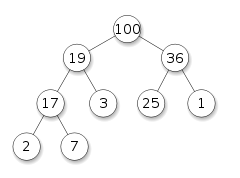
\includegraphics[height=32mm]{heap.png}
\caption{Max-heap Example from Wikipedia}
\end{figure}
\begin{itemize}
\item insert node with certain key value: $O(\log n)$
\item find node with min(max) key value: $O(1)$
\item update key value of certain node after the node is located: $O(\log n)$
\item remove node with min(max) key value: $O(\log n)$
\item find node with {\bf arbitrary} key value: $O(n)$
\end{itemize}
\end{frame}

\begin{frame}
\frametitle{Heaped APS}
\framesubtitle{$O(1)$ Query for Arbitrary Key Value in Heap}
\begin{figure}[ht]
\centering
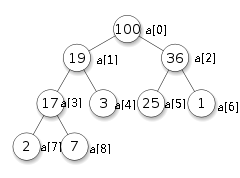
\includegraphics[height=32mm]{heap2.png}
\end{figure}
\begin{itemize}
\item The two children nodes of node $a[i]$ can be represented as $a[2 \times i + 1]$ and $a[2 \times i + 2]$, if exists.
\item Track internal location of each node!
\end{itemize}

\end{frame}

\begin{frame}
\frametitle{Heaped APS}
\framesubtitle{Heaped Comparing}
$$ \bar{X_{i}}(N_{ir}) - \bar{X_{j}}(N_{jr}) < \min\{0, -\frac{a}{\delta}[\frac{S_i^2(N_{ir})}{N_{ir}} + \frac{S_j^2(N_{jr})}{N_{jr}}] + \frac{\delta}{2}\} $$
\begin{itemize}
\item To see whether $ -\frac{a}{\delta}[\frac{S_i^2(N_{ir})}{N_{ir}} + \frac{S_j^2(N_{jr})}{N_{jr}}] + \frac{\delta}{2} > 0$, just check largest $\frac{S^2(N_r)}{N_r}$.
\end{itemize}
$$ \bar{X_{i}}(N_{ir}) - \bar{X_{j}}(N_{jr}) < -\frac{a}{\delta}[\frac{S_i^2(N_{ir})}{N_{ir}} + \frac{S_j^2(N_{jr})}{N_{jr}}] + \frac{\delta}{2} $$
$$ \bar{X_{i}}(N_{ir}) + \frac{a}{\delta}\frac{S_i^2(N_{ir})}{N_{ir}} < \bar{X_{j}}(N_{jr}) - \frac{a}{\delta}\frac{S_j^2(N_{jr})}{N_{jr}} + \frac{\delta}{2} $$
\begin{itemize}
\item Check smallest $\bar{X}(N_r) + \frac{a}{\delta}\frac{S^2(N_r)}{N_r}$, with iteration.
\item Check largest $\bar{X}(N_r) - \frac{a}{\delta}\frac{S^2(N_r)}{N_r}$, without iteration.
\end{itemize}
\end{frame}

\begin{frame}
\frametitle{Heaped APS}
\framesubtitle{Heaped Comparing Algorithm}
\begin{algorithmic}[1]
\tiny
{
\Require $simOutput$, including corresponding $altId$ and $value$ of output
\State $alt = alts0[altId]$ \Comment{$alts0$ is an array of alternative objects, $O(1)$}
\If{$alt.isSurviving() = false$} 
  \State \Return
\EndIf
\State $alts.addSample(value)$ \Comment{update $N, \bar{X}(N), S^2(N)$ e.g. $O(1)$}
\State adjust heap $alts1$, $alts2$, $alts3$, where $alts1$ is a max-heap with key $S^2(N)/N$, $alts2$ is a min-heap with key $\bar{X}(N) + \frac{a}{\delta}\frac{S^2(N)}{N}$, $alts3$ is a max-heap with key $\bar{X} - \frac{a}{\delta}\frac{S^2(N)}{N}$, the complexity is $O(\log k)$
\State $alt1 = alts1.peek()$
\While {$alt.key1() + alt1.key1() < \frac{\delta^2}{2a}$}
  \If{alt.mean() < alt1.mean()}
    \State eliminate $alt$ and \Return \Comment{heap adjustment involved, $O(\log k)$}
  \Else
    \State eliminate $alt1$ and $alt1 = alts1.peek()$ \Comment{heap adjustment involved, $O(\log k)$}
  \EndIf
\EndWhile
\State $alt2 = alts2.peek()$
\While{$alt2.key2() < alt.key3()$}
  \State eliminate $alt2$ and $alt2 = alts2.peek()$ \Comment{heap adjustment involved, $O(\log k)$}
\EndWhile
\State $alt3 = alts3.peek()$
\If{$alt.key2() < alt3.key3()$}
  \State eliminate $alt$ and \Return \Comment{heap adjustment involved, $O(\log k)$}
\EndIf
}
\end{algorithmic}
\end{frame}

\begin{frame}
\frametitle{Heaped Comparing Algorithm}
\framesubtitle{Substantial Accelaration of Serial Part}
\begin{itemize}
\item {Alternative: } normal distributed simulation result, with pre-known mean and variance
\item {Configuration: } increasing number of alternatives, one of them has max-mean 1, others has mean of 0. Variance is 1.
\item {Environment: } pc with 8 hardware thread, using 4 slaves. $\alpha=0.05, \delta=1, n_0 = 10$.
\item {Result: } $100\%$ correct selection.
\end{itemize}
\begin{table}[ht]
\begin{center}
\begin{tabular}{|c|c|c|c|c|c|c|}
\hline
Num. of Alternatives(k): & 100 & 1000 & 10000 & 100000 \\
\hline
Linear Comparison (ms): & 56 & 199.6 & 5606.4 & 884992.6 \\
\hline
Heaped Comparison (ms): & 54.8 & 163.6 & 906 & 10338.6 \\
\hline
\end{tabular} \\
\caption{Effect of Heaped Comparison}
\end{center}
\end{table}
\end{frame}

\section{Conclusion and Future Work}

\begin{frame}
\frametitle{Conclusion}
\begin{itemize}
\item We pay attention to not only statistical validity, but also computational time complexity and scalability.
\vspace{\baselineskip}
\item Our extensible framework has achieved a good scalability with most workload being carried out in parallel.
\vspace{\baselineskip}
\item Our comparison algorithm inside the serial part of our system, has achieved time complexity of $O(\log n)$, which has further improved the performance of the whole system.
\end{itemize}
\end{frame}

\begin{frame}
\frametitle{Related Work}
\begin{itemize}
\item simulation R\&S procedure: traditionally focus on statistical validity
\vspace{\baselineskip}
\item parallel and distributed simulation(PADS): accelerating single extremely long simulation experiment
\vspace{\baselineskip}
\item optimization via simulation(OvS): sacrificing statistical validity for dealing with larger problem size in serial computing environment
\end{itemize}
\end{frame}

\begin{frame}
\frametitle{Future Work}
\begin{itemize}
\item system viewpoint
\begin{itemize}
\item architecture: centralized v.s. decentralized (see \cite{potwsc05ras})
\item task scheduling: task-pool v.s. explicit scheduler
\end{itemize}
\item implementation viewpoint
\begin{itemize}
\item algorithm complexity: more rigorous analysis of heaped comparing
\item sample processing: single v.s. batched
\end{itemize}
\item application viewpoint
\begin{itemize}
\item we lack a comparative study of parallel procedures (see \cite{ms05ras})
\item providing service as cloud computing and become benchmark
\end{itemize}
\item others
\begin{itemize}
\item we lack a thread-safe discrete-event simulation library (see \cite{ssj})
\end{itemize}
\end{itemize}
\tiny
{
\begin{thebibliography}{10}
\bibitem{potwsc05ras} Chen, E. J. Using parallel and distributed computing to increase the capability of selection procedures. In Proceedings of the 2005 Winter Simulation Conference, pp. 723–731.
\bibitem{ms05ras} Jurgen Branke, Stephen E. Chick, Christian Schmidt. Selecting a Selection Procedure. Management Science, 2005.
\bibitem{ssj} Lecuyer Pierre, Simard Richard, Chen E. Jack, Kelton W. David. An Object-Oriented Random-Number Package with Many Long Streams and Substreams. Operations Research, 2002.
\end{thebibliography}
}
\end{frame}

\begin{frame}
\begin{center}
\Huge \bf \color{blue} THANK YOU!
\end{center}
\end{frame}

\end{document}
